
\iffalse \section{Visualizacion de datos}

La visualización de datos es la práctica de traducir información en un contexto visual, como un mapa o gráfico, para facilitar que el cerebro humano comprenda y extraiga información útil.\\

Las formas más generales de visualización de datos son las siguientes: Gráficas, Tablas, Mapas, Infografias y Tableros. En este trabajo se hará uso especificamente de gráficas como medio de visualización de datos, ya que los datos obtenidos de Wikipedia no permiten ser visualizados de otra forma.


\subsection{Tipos de gráficas} \fi

\section{Dominio del problema}
    \subsection{Wiki, Mediawiki y Wikimedia}

        El término wiki proviene de la raíz Hawaiana \say{wiki}, que significa \say{rápido}, y fue propuesto por Ward Cunningham, quien a su vez define los sitios web wiki como "La base de datos más simple que puede existir" [Cunningham, Ward (June 27, 2002), What is a Wiki]. Con el tiempo este concepto fue evolucionando, y en la actualidad cuando hablamos de wiki nos referimos a un sitio web que permite a sus usuarios colaborar en su estructura y contenido. Estos sitios webs son impulsados por el motor wiki, tambien llamado MediaWiki, el cual es un Sistema Manejador de Contenido (CMS) que permite a los usuarios colaborar en el sitio web sin la necesidad de tener permisos de dueño o lider. \\

        La enciclopedia Wikipedia es el sitio web más popular basado en wiki, que a su vez forma parte del movimiento Wikimedia, el cual incluye otros proyectos interrelacionados, tales como: Wiktionary, Wikiquote, Wikibooks, Wikisource, entre otros, cuyo propósito es usar el poder colaborativo de internet, y el concepto wiki, para compartir conocimiento gratuito de cualquier tipo.\\
     
    \subsection{Filosofía de wiki}

        \iffalse \input{[https://www.um.es/ead/red/M11/intro.pdf]
        [https://ignasialcalde.es/filosofia-wiki-y-dinamicas-relacionales/]} \fi
        
        En la actualidad, gracias a la evolución del internet, la información es considerada virtualmente ubicua y en constante cambio, y lo que realmente ofrece valor es la capacidad individual de sintetizar esa información y relacionarla. Como resultado de esto surge la filosofía wiki, en donde la información se comparte, y el conocimiento no se crea, sino se co-crea de forma colaborativa. \\

        El concepto de la filosofía de wiki y el software utilizado para crear estos sitios web estan intrínsecamente relacionados, y no se podría poner en práctica lo primero sin lo segundo. Esto es así debido a que el software debe proporcionar el medio para que pueda existir esa construcción colectiva de conocimiento, que es indispensable en la filosofía wiki.\\
        
        Algunas de las características de software de los sitios web que hacen uso de esta filosofía son: 
    
        \begin{enumerate}
            \item Cualquiera puede cambiar cualquier cosa
            \item Usan un sistema de marcas hipertextuales simplificadas, lo que resulta imprescindible para hacer posible la colaboración.
            \item No posee una estructura predefinida a la que se tengan que acomodar los usuarios, lo que otorga flexibilidad.
        \end{enumerate}

        \subsection{Moderación de contenido en Wikipedia}

        \iffalse \input{https://design.wikimedia.org/blog/2020/07/30/content-moderation-anti-vandalism-wikipedia.html} \fi

        El principal problema que maneja Wikipedia en cuanto a moderación de contenido viene como resultado de su propia filosofia de "todos pueden editar", lo que conlleva a multiples problemas tales como: vandalismo, escritura pobre, una mala estructura de página, peleas de edición, entre otras cosas. Por esta razón no existe una solución única para acabar con la existencia de "mal" contenido en Wikipedia, y es indispensable el uso de participación humana en procesos de moderación que implican complejos desafíos técnicos y éticos.\\

        Una de las formas que tiene Wikipedia de detectar vandalismo es usando las estadisticas de los articulos para verificar si hay una gran cantidad de ediciones de un articulo en un periodo muy corto de tiempo, o si estas revisiones vienen de la misma dirección IP, bloqueando o baneando las direcciones IP como método de reducción de vandalismo. Sin embargo, el bloqueo de IPs es en sí mismo un método que resulta contradictorio para el nucleo principal de la filosofia de wiki: "todos pueden editar".

        
        \subsection{Watcher}


       
    \subsection{Wikipedia como ejemplo práctico}

    \subsection{Visualizacion cientifica}


\subsection{Tecnologias a utilizar}

    Para la realización de este proyecto se usarán las siguientes tecnologías:

    \subsubsection{ReactJS}

        ReactJS es una librería de JavaScript de código abierto desarrollada por Facebook para facilitar la creación de componentes interactivos, reutilizables, para desarrollos de interfaces de usuario, especialmente aplicaciones de una sola página.

        React maneja el concepto de \say{programación reactiva} haciendo uso de un DOM Virtual, lo le permite determinar qué partes del DOM han cambiado comparando contenidos entre la versión nueva y la almacenada den el DOM virtual, para así propagar los datos generando cambios en la aplicación, es decir, los datos \say {reaccionan} ejecutando una serie de eventos.

        \iffalse 
            \begin{figure}
                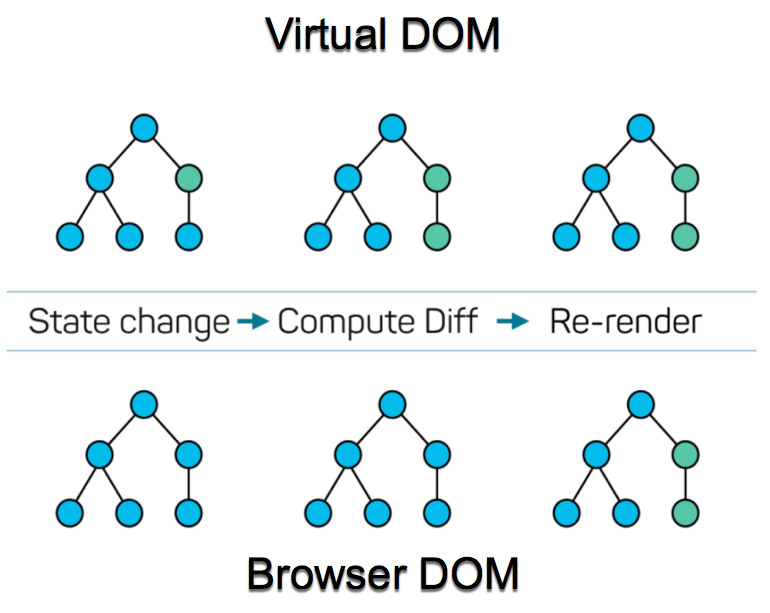
\includegraphics[scale=0.5]{virtual_dom}
                \caption{Propagación de datos usando el Virtual DOM}
            \end{figure}
        \fi

        Este concepto de reactividad es lo que hace a la libreria altamente eficiente, ya que limita la actualización del DOM solamente a los elementos que han cambiado.
        
    \subsubsection{SEO}
    
        Se trata del proceso de mejorar un sitio web en relación con los motores de búsqueda. También representa el cargo de la persona que trabaja en este proceso: Acabamos de contratar a un nuevo SEO para que mejore nuestra presencia en la Web.

    \subsubsection{NextJS}

        NextJS es un framework desarrollado encima de Node.js que permite a las aplicaciones de React usar funcionalidades como el renderizado del lado de servidor o la generación estática de paginas, que permite realizar aplicaciones con mejor desempeño en cuanto a SEO.


    \subsubsection{Mongo}

        MongoDB es un sistema de base de datos NoSQL, orientado a documentos y de código abierto. En lugar de guardar los datos en tablas, tal y como se hace en las bases de datos relacionales, MongoDB guarda estructuras de datos BSON (una especificación similar a JSON) con un esquema dinámico, haciendo que la integración de los datos en ciertas aplicaciones sea más fácil y rápida.

        \iffalse 
            \begin{figure}
                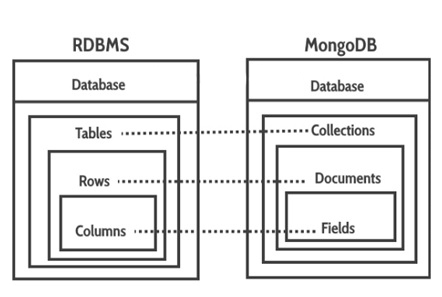
\includegraphics[scale=1.2]{mongodb-structure.jpg}
                \caption{Comparación de estructura de datos entre MongoDB y los RDBMS (sistema de gestión de bases de datos relacionales)}
            \end{figure}
        \fi

    \subsubsection{Fastify}



\subsection{Metodologias agiles}


    \subsubsection{Frameworks}

    \begin{enumerate}
        \item Kanban: Tiene como objetivo la mejora continua, la flexibilidad en la gestión de tareas y un flujo de trabajo mejorado. Con este enfoque ilustrativo, el progreso de todo el proyecto se puede comprender fácilmente de un vistazo. Para esto hace uso del tablero Kanban, que es una herramienta que visualiza todo el proyecto para rastrear el flujo de su proyecto. A través de este enfoque gráfico de los tableros Kanban, un miembro nuevo o una entidad externa puede comprender lo que está sucediendo en este momento, las tareas completadas y las tareas futuras.
        \item Scrum: Es un framework para desarrollo, entrega, y mantenimiento de proyectos en un ambiente complejo, con un enfasis inicial en el desarrollo de software, aunque tambien ha sido utilizado en otras areas como la investigación, ventas, mercadeo y tecnologías avanzadas. Esta diseñado para equipos de 10 personas o menos, quienes rompen su trabajo en metas que pueden ser completadas en iteraciones de tiempo fijo, llamadas \emph{sprints}, con duraciones aproximadas de 2 semanas. 
        \item Lean software development: Es un framework popular basado en optimizar tiempo de desarrollo y recursos, eliminando desperdicios y entregando solamente lo que el producto necesita. El método Lean es usualmente referido como la estrategia del \say{Producto Minimo Viable (PMV)}, 
        estrategia, en la que un equipo lanza una versión mínima de su producto al mercado, aprende de los usuarios lo que les gusta, lo que no les gusta y lo que quieren que se agregue, y luego itera en función de estos comentarios.
        \item Extreme programming (XP)
        \item Adaptive Software Development (ASD):
        \item Rapid application development (RAD)
    \end{enumerate}

    \subsubsection{Prácticas}

    \begin{enumerate}
        \item Backlogs (Product and Sprint)
        \item Continuous integration (CI)
        \item Daily Stand-up / Daily Scrum
        \item Domain-driven design (DDD)
        \item Acceptance test-driven development (ATDD)
        \item Iterative and incremental development (IID)
        \item Planning poker
        \item Refactoring
        \item Pair programming
        \item Specification by example
        \item Story-driven modeling
        \item Test-driven development (TDD)
    \end{enumerate}

